\documentclass[12pt]{article}
\usepackage{listings}
\usepackage{hyperref}
\usepackage{graphicx}
\usepackage{float}
\title{EARIN project Final report}
\author{Krzysztof Rudnicki \\ Jakub Kliszko}
\begin{document}
\maketitle
\section{Introduction}
The goal of our project was to create a model for anime recommender \\ 
After entering anime name from the database model should output recommended anime's 
\section{Used data and algorithms}
\subsection{Data}
We used different data-set from originally specified in the project description \\ 
We decided to use Anime Recommendation Database from Kaggle: \href{https://www.kaggle.com/datasets/hernan4444/anime-recommendation-database-2020}{LINK} \\ 
Main reasons why we decided to use this database was that it was bigger than original one, was more recent, it was described as being 100\% usable by Kaggle and still had decent amount of code examples \\ 
We are mostly interested in rating\_complete.csv file which contains information about anime ratings from users who completed the anime 
\subsection{Algorithms}
We decided to use collaborative filtering to develop our model, It makes personalized recommendations based on preferences of similar users \\ 
We represent anime data-set as embedding vector \\ 
We use K-nearest neighbors model and decided to test it out with different metrics, neighbors and algorithms \\ 
\subsubsection{Algorithms}
We decided to test our model with 2  algorithms:
\begin{enumerate}
  \item Brute
  \item Auto
\end{enumerate}
Ball Tree and KD Tree do not work on sparse input (as is the case with our input) so we decided to omit them

\subsubsection{Neighbor number}
We decided to test our model with 5 different neighbor amount:
\begin{enumerate}
  \item 5 - Popular starting point for small-medium data-sets
  \item square root of available data - Usually helps to balance between under-fitting and over-fitting
  \item half of available data - Usually useful for checking overall trend than specific nuances 
  \item logarithm of available data - Used for very large data-sets
  \item n-1 neighbors - Usually leads to over generalization as we use all instances except one for prediction
\end{enumerate}

\subsubsection{Metrics}
For brute algorithm we tested it will all possible metrics:
\begin{enumerate}
  \item Cosine - Measures cosine of angle between vectors 
  \item Euclidean - Measures distance in straight line between two points
  \item Manhattan - Measures sum of absolute paths between two coordinates 
\end{enumerate}

\section{Intermediate results}
\subsection{Results}
For intermediate solution we have implemented reading data from csv files, preprocessing them with optional showing of some of the information about the data and used model/learner for implementing neighbour searches \\ We implemented full manual mode for our program and added some parameters that will be later used for auto mode like choosing type of metric, algorithm, number of neighbors and seed
\subsection{Insights}
We find out that the solution we wanted to initially base on: \href{https://www.kaggle.com/code/chaitanya99/recommendation-system-cf-anime}{Kaggle code with tensorflow} was too complicated and required too much computational time, so we changed it to a simpler, faster one that was still enough to provide the solution \\ 
We also found out when investigating the ratings that the rating is skewed towards higher values like 7, 8, 9 so the average rating is well above 5 
\begin{figure}[H]
  \caption{User rating count}
  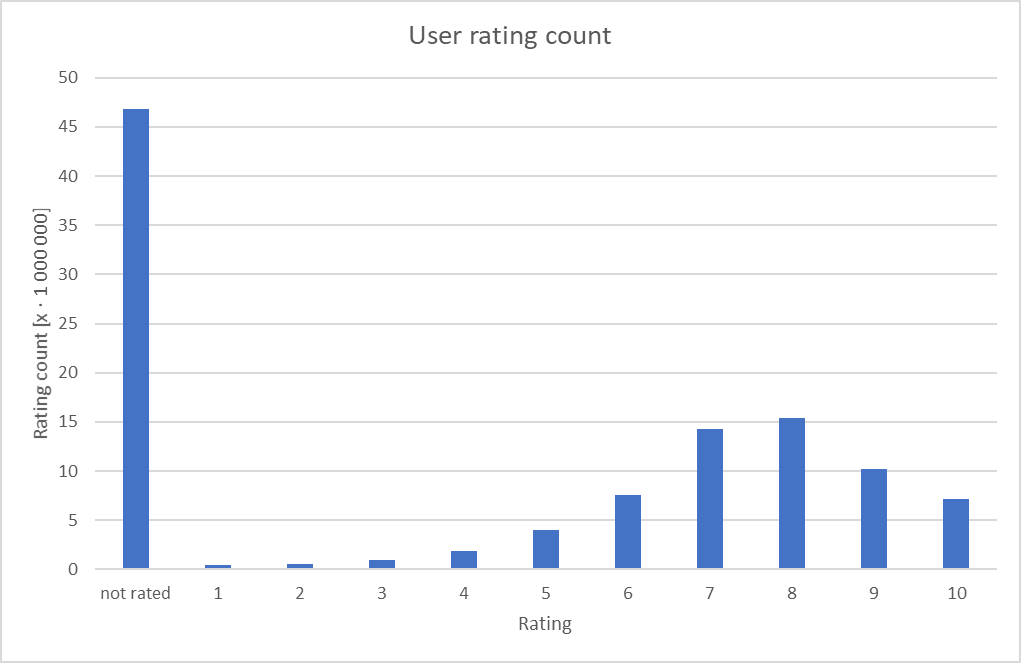
\includegraphics[width=\textwidth]{user_rating.png}
\end{figure}

\section{Using program} 
  \subsection{Arguments}
  There are 13 parameters that can be modified which either influence how the program behaves or how the model behaves, too see how they can be modified user needs to run 
  \begin{lstlisting}[language=bash]
    python main.py -h
  \end{lstlisting}
  Command    
  \begin{lstlisting}[language=bash]
    options:
  -h, --help            show this help message and exit
  --data_limit DATA_LIMIT, -dl DATA_LIMIT
                        Specify data limit,
                        Recommended at least 500k,
                        set to -1 for no limit
  --seed SEED, -s SEED  Specify seed
  --debug DEBUG, -d DEBUG
                        Use debug (more information) prints
  --database DATABASE, -db DATABASE
                        Specify database path
  --metric {cosine,mahalanobis,euclidean},
  -m {cosine,mahalanobis,euclidean}
                        Specify metric for NearestNeighbor learner
  --algorithm {auto, brute},
  -a {auto, brute}
                        Specify algorithm for
                        Nearest Neighbor learner
  --anime ANIME, -an ANIME
                        Specify anime to choose
  --neighbors NEIGHBORS, -n NEIGHBORS
                        Specify number of nearest neighbors
  --user_threshold USER_THRESHOLD, -ut USER_THRESHOLD
                        Specify minimal number of votes required for
                        user to be included in the data, set to -1 for
                        no threshold
  --anime_threshold ANIME_THRESHOLD, -at ANIME_THRESHOLD
                        Specify minimal number of votes required for
                        anime to be included in the data, set to -1 for
                        no threshold
  --recommendation_amount RECOMMENDATION_AMOUNT,
  -ra RECOMMENDATION_AMOUNT
                        Specify how much anime should be recommended
  --auto AUTO, -au AUTO
                        Enable auto mode, no debug,
                        no user parameters, automatic testing and saving results
  \end{lstlisting}
    \subsubsection{Default arguments}
    Default values of arguments are:
    \begin{itemize}
      \item Data Limit = -1 (means no limit, all data will be used)
      \item Seed = 42
      \item Debug = False (means no debug information will be shown)
      \item Database = database 
      \item Metric = cosine
      \item Algorithm = brute
      \item Anime = RANDOM (program will randomly choose anime for which there should be recommendation)
      \item Neighbors = 5
      \item User Threshold = 500
      \item Anime Threshold = 200 
      \item Recommendation Amount = 5
      \item Auto mode = False
    \end{itemize}
    \subsubsection{Reproducing}
    In order to reproduce test results user should use:
    \begin{lstlisting}
      python main.py -au True -dl 600000
    \end{lstlisting}
    Command which will run auto mode with 600 thousand entries
      

\section{Final experimental results}
\subsection{Experiments}
All of our experiments were done on data limited to \textbf{600 thousand entries}, rest of parameters were default \\ 
We checked for 2 things in our experiments, precision of our algorithm and distances between recommended anime and input anime for different metrics and number of neighbors \\ 
Precision was calculated based on the rating of anime which was recommended, if the anime recommended had rating higher or equal to 8 then the recommendation was "good", so true positive is any anime which rating is above or equal to 8 \\ 
Unfortunately we did not manage to calculate recall and F1 score (since it requires recall to be calculated)
\subsection{Results}
\subsubsection{Precision}
\begin{figure}[H]
  \caption{Precision from different metrics and auto algorithm}
  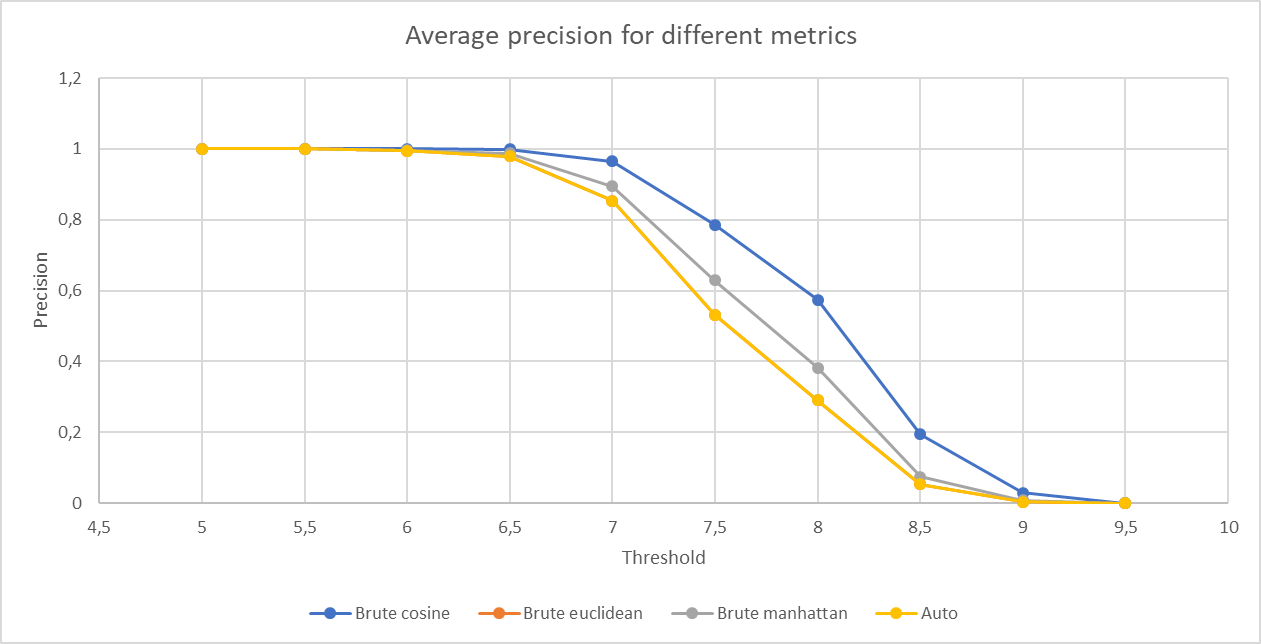
\includegraphics[width=\textwidth]{precision_metric.png}
\end{figure}
\begin{figure}[H]
  \caption{Precision from number of neighbors}
  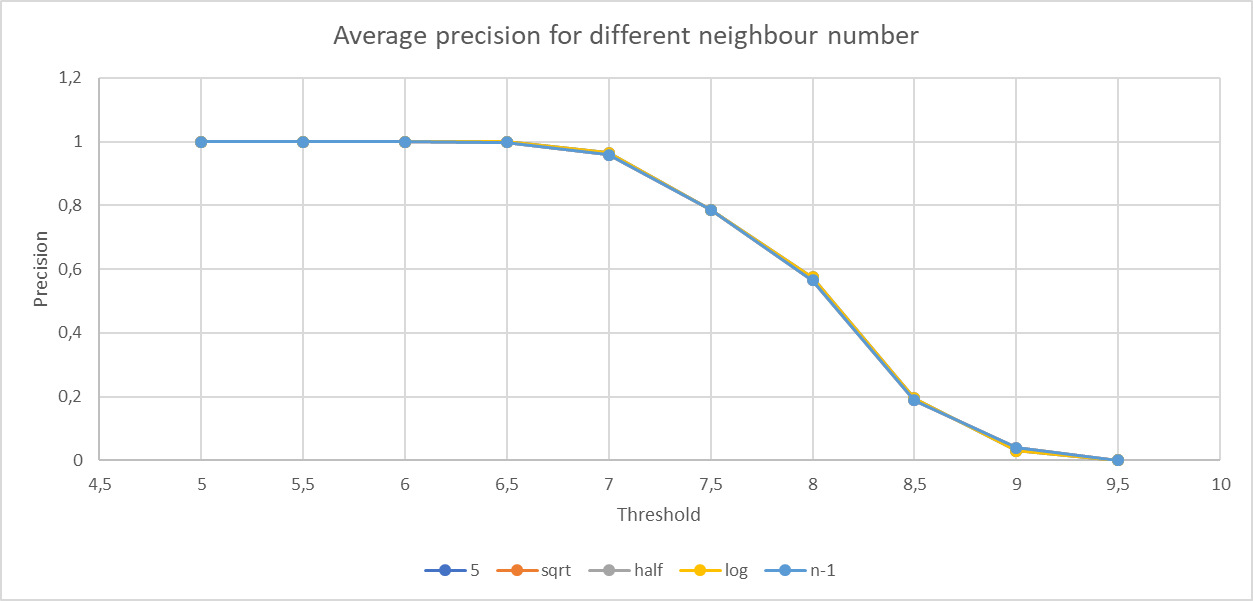
\includegraphics[width=\textwidth]{precision_neighbor.png}
\end{figure}
\subsubsection{Distance}
\begin{figure}[H]
  \caption{Distance for Manhattan}
  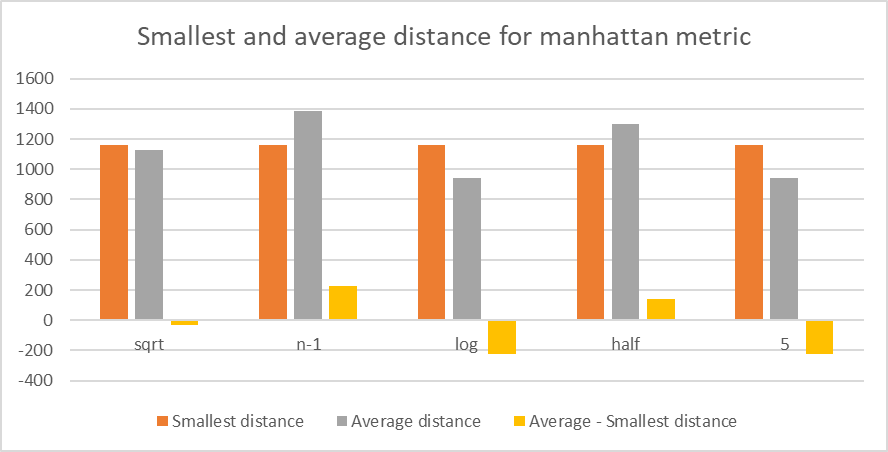
\includegraphics[width=\textwidth]{distance_manhattan.png}
\end{figure}
\begin{figure}[H]
  \caption{Distance for Euclidean}
  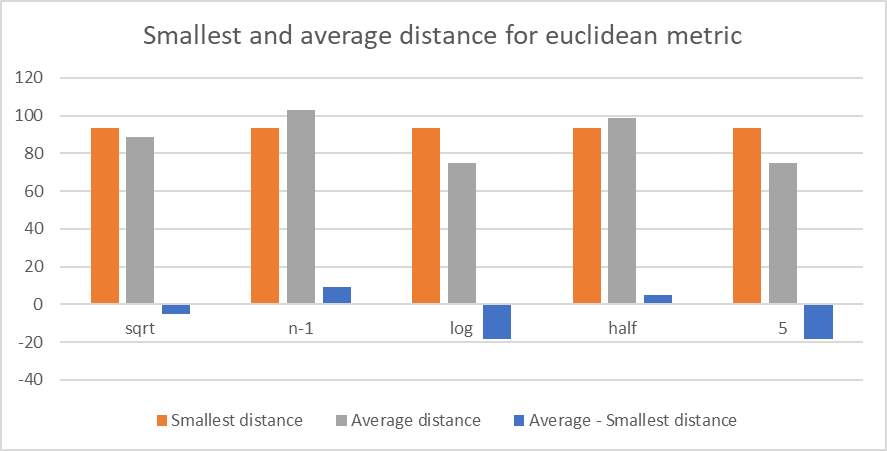
\includegraphics[width=\textwidth]{distance_euclidean.png}
\end{figure}
\begin{figure}[H]
  \caption{Distance for Cosine}
  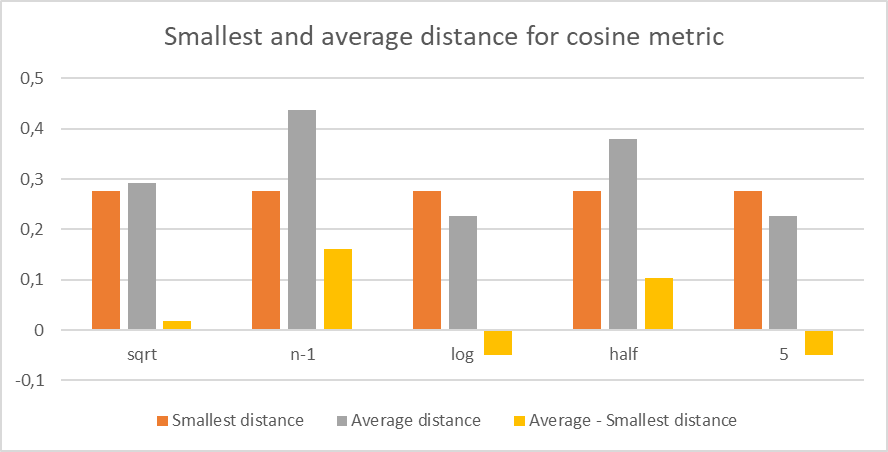
\includegraphics[width=\textwidth]{distance_cosine.png}
\end{figure}
\begin{figure}[H]
  \caption{Distance for Auto mode}
  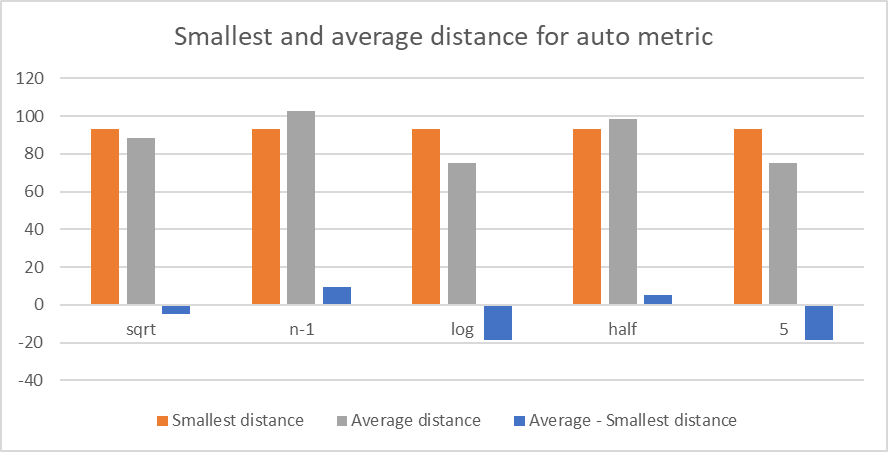
\includegraphics[width=\textwidth]{distance_auto.png}
\end{figure}
\subsection{Discussion}
\subsubsection{Precision}
As expected number of neighbors does not have influence on precision, metric used on different hand does, as we can see cosine metric achieves the best precision compared to cosine and euclidean metric. \\ 
This means that the anime that is recommended from a model that metric usually has higher rating than anime's that use euclidean or Manhattan metric. \\
Auto mode seems to use euclidean metric as the results between those two are exactly the same
\subsubsection{Distance}
Smallest distance was always the same within the same metric no matter the number of neighbors used \\ 
The only thing that changed was average distance and consequently difference between average distance and smallest distance \\ 
In general smaller number of neighbors used meant smaller average distance, notice how for neighbors equal to 5 and logarithm of number of entries average distance in all charts is roughly the same and below average distance for number of neighbours equal to square root of entries, half of entries or all entries but one \\ 
We think that it means that simply by taking more data into consideration when recommending anime we increase number of outliners that are radically "far" from input anime \\ 
For some reason sometimes the average distance was actually smaller than smallest distance, we did manage to understand why within time limit of this project \\ 


\section{Challenges}
\subsection{Challenges themselves}
\paragraph{Precision}
The biggest challenge was implementing the algorithm that checks precision of our model, we had to reject recall and F1 score since defining what sort of base should they use to measure correctness of solution was not a trivial task
\paragraph{Data Size}
Another challenge was with the size of database itself which impacted speed of running new changes 
\paragraph{Visualisation}
It was not easy to visualize the effects of experiments themselves, most program output is simple text and there is not much continues data that naturally aligns itself with some graphs
\subsection{Tackling challenges}
For precision we just settled on the idea of good recommendation to be any recommendation that recommends anime with rating above or equal 8 \\ 
For Data size we introduced data limit argument which made it very easy and fast to introduce new changes \\ 
For visualization we agreed on going through the precision of algorithm based on different thresholds and showing data for distances in the histogram chart

\section{Conclusions}
\paragraph{Best parameters}
For our precision metrics we lean towards brute algorithm with cosine metric used, probably with logarithmic or 5 number of neighbors \\ 
Cosine metric provides us with the best precision and small number of neighbors offers smaller average distance, it also behaves as expected since the average distance is smaller than the distance between input anime and recommended anime
\subsection{Solution satisfaction}
Our solution works, it manages to go through entire data-set and return some recommendation \\ 
Those recommendation based on manual inspections are usually OK, model often behaves rationally for example by recommending sequel of anime when given anime's first part \\ 
We also manage to make basic precision algorithm which considering how hard it is to define what a "correct" recommendation is, should be considered a success \\ 
Overall we are content with the result given limited time, knowledge and resources on our disposal
\subsection{Potential improvements}
We did not manage to introduce more parameters when embedding data into vectors, like anime popularity or how controversial it is, this would probably make the model at least more interesting if not directly better

\end{document}